\chapter{Preliminaries}
\label{ch:Preliminaries}
\lettrine[lraise=-0.1, lines=2, loversize=0.2]{T}{his} chapter focuses on the current state of the art of those technologies related to this project, as well as on the tools used for the development of the task planner as a software layer of a multi-layer architecture. In addition, the research work carried out on the state of the art in work related to the technologies and techniques used in this project is presented. 

% Poner en contexto las tecnologías que hay hoy día y demás.
\section{Current technology}
\label{sec:CurrentTechnology}
%% Origen de los drones (vehículos aéreos no tripulados, controlados por radiocontrol, no son autonomos, forma tipica de aeronave).
Although in the last decade the use of \glspl{UAV} has spread to a large number of applications, the origin of this technology dates back to 1898 with the invention of radio control and the appearance of the first unmanned aircraft, baptised with the name of drone. These were not yet unmanned aerial vehicles, and were mainly used for military purposes.

\begin{figure}[htbp]
    \centering
    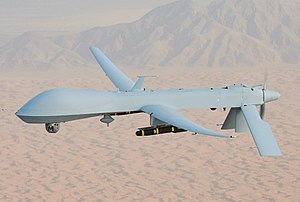
\includegraphics[width=0.6\linewidth]
    {Preliminaries/figures/Predator.jpg}
    \caption{General Atomics MQ-1 Predator. A \gls{RPA}. Source: \href{https://en.wikipedia.org/wiki/General_Atomics_MQ-1_Predator}{Wikipedia}}
    \label{fig:predator}
\end{figure}

%% Primeros UAV (drones autónomos). 
Later, with the development of technology, the first computers of sufficient size and computing power to run the software necessary to operate a \gls{UAV} autonomously and even to control aircraft with more complex and even unstable dynamics (gliders \cite{predator, BIGBLUE}, airships \cite{AURORA}, quadrotors \cite{quadrotorsreview, mesicopter, pounds, miniquadrotor}, multirotors \cite{fullyactuated}, flapping wings \cite{COLIBRI, GRIFFING, GRIFFIN2021}, etc.) appeared. Even though computational capacity was still insufficient for some applications, the development of \gls{UAV} systems was made possible by performing calculations on the ground. What was done was to run the critical and most important systems for autonomous flight on the on-board computer (controls, data acquisition, obstacle avoidance, etc.), and to run the more demanding calculations that are not necessary in real time on the ground computers \cite{OffBoard}.

\begin{figure}[htbp]
    \centering
    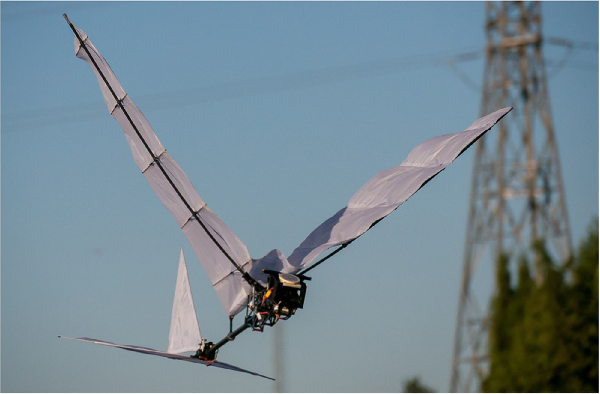
\includegraphics[width=0.6\linewidth]
    {Preliminaries/figures/GRIFFIN.png}
    \caption{GRIFFIN's flapping wing robot \cite{GRIFFIN2021}}
    \label{fig:predator}
\end{figure}

%% Adquisición de datos (para ser autónomos necesitan recolectar datos del entorno)
For an aerial vehicle to operate autonomously, it is necessary to acquire data from the environment and process it in real time. A large number of different sensor configurations as well as numerous data acquisition and processing techniques can be found in the current literature \cite{SenseAndAvoid, aasen2018quantitative, miningSensors}.

%% Aplicaciones para UAV existentes (que necesitan de un piloto humano que supervise, no son cognitivos)
%% Equipos multi-UAV (con supervisión humana) [multiUAVclassification]
%% Explosión de la tecnología.
Once UAV technology reached sufficient capacity and autonomy, the first applications for both single \cite{nex2014uav, radoglou2020compilation, drummond2015uav} and multi-\gls{UAV} \cite{martinez2007multi, gu2018multiple, scherer2015autonomous} equipment began to appear. There is great interest in the latter, as they can be configured in different ways \cite{multiUAVclassification}, collect and process data in a distributed way, increasing the computational capacity of the equipment \cite{pascarella2015parallel, guo2021coded}, and generate global collective behaviour emerging from interactions between a large number of \glspl{UAV} that individually are relatively simple, known as swarming \cite{zhou2020uav, campion2018uav, chen2020sidr}. 

%% Esfuerzo para el desarrollo de aplicaciones sin presencia humana: capacidades cogitivas, entornos dinámicos. (Aerial co-workers)
Current applications often require human presence to carry out certain decisions, with the human pilot overseeing that everything runs smoothly and providing the cognitive capacity to analyse the generally dynamic environment and react to unforeseen situations \cite{sebbane2015smart, MITfullyAutonomous,kopeikin2012flight}. This is because providing a \gls{UAV} with sufficient cognitive capacity to operate fully autonomously in dynamic environments is a very complicated task and requires a great deal of processing power. In recent years, \gls{UAV} technology has evolved rapidly, benefiting from advances in computing and artificial intelligence. As processors are becoming more powerful, efficient and smaller, \glspl{UAV} are becoming more and more powerful without increasing their weight or compromising their autonomy. With the increase in the number of operations per second that \glspl{UAV} can perform, this opens up the possibility of using drones for previously unthinkable applications, applications that require a large amount of processing and usually have to be performed in real time \cite{CivilAplications, shakeri2019design}. At the same time, advances in artificial intelligence mean that the perception, analysis and sensory fusion capabilities of \glspl{UAV} are getting better and better. Advances in technology are breaking down one of the barriers preventing \gls{UAV} technology from achieving this level of autonomy, and with it, more and more research effort is being devoted to breaking down the other barrier, developing software that enables \glspl{UAV} to have cognitive capabilities.

%% Investigaciones recientes para aplicaciones 100% autónomas
% Aerial Co-workers
% Mencionar proyectos en los que está involucrada la universidad de sevilla
Mentioning some of the research that is currently being carried out, we can recall the well-known AERIAL-CORE European project\footnote{AERIAL-CORE European project homepage: \url{https://aerial-core.eu/}}, in which major European robotics teams are jointly participating with the aim of developing a fully autonomous robotic system with sufficient cognitive capabilities to work together with human operators in inspection and maintenance work on electrical networks \cite{cacace2021safe}. The PILOTING European project\footnote{PILOTING European project homepage: \url{https://piloting-project.eu/}} aims to develop a complete inspection platform that will provide its users with the information they need to draw up maintenance plans for structures \cite{benjumea2021localization}. HYFLIERS \footnote{HYFLIERS European project homepage: \url{https://www.oulu.fi/hyfliers/}} is a completed European project that focused on the inspection of long pipe arrays in hard-to-reach areas. This, unlike the previous two, is not fully autonomous, but needs a pilot to indicate the inspection points along the pipes, and to supervise the aerial robot while it operates \cite{suarez2020aerial}. It is also worth mentioning a recent \acrshort{NASA} (\acrlong{NASA}) achievement, which is no less than the first flight of an \gls{UAV} outside the Earth \cite{schroeder2020nasa, potter2020mars}. This is specifically the Martian helicopter called Ingenuity, whose mission was simply to take off, move around and land in the Martian atmosphere with the added difficulty that, due to the distance between the two planets, this had to be done completely autonomously.

% Related work: buscar artículos que tengan que ver con mi proyecto para poner en contexto lo que voy a aportar.
\section{Related work}
\label{sec:RelatedWork}
%% Parrafo de introducción del trabajo relacionado con el mío: planificador de tareas cognitivo
% Volver a hablar de UAV para inspección, centrandose en multi-UAV y explicar la necesidad de diseñar planificadores cognitivos. Enumerar las partes de las que se compone el planificador diseñado a modo de enlace con los siguientes párafos 

%% Task planning in multi-drone teams 
% Hablar de las formas existentes que hay para abordar el problema del reparto de tareas en equivos multi-UAV. Poner en contexto lo que voy a aportar con mi TFM.

%% Drone behavior management
% Hablar de las formas existentes que hay para gestionar el comportamiento de un dron y su guiado en cada instante. Poner en contexto lo que voy a aportar con mi TFM. Hablar de las FSM y de los BT

% Capi: quitar las subsecciones si veo que se puede integrar todo junto. Si veo que queda largo, dividir en subsecciones como tengo.
\subsection{Inspection applications with UAVs}
\label{subsec:InspectionApplicationsWithUAVs}

% Hablar de las formas existentes que hay para abordar el problema del reparto de tareas en equivos multi-UAV. Poner en contexto lo que voy a aportar con mi TFM.
\subsection{Task planning in multi-drone teams}
\label{subsec:TaskPlanning}

% Hablar de las formas existentes que hay para gestionar el comportamiento de un dron y su guiado en cada instante. Poner en contexto lo que voy a aportar con mi TFM. Hablar de las FSM y de los BT
\subsection{Drone behavior management}
\label{subsec:DroneBehaviorManagement}


% Estudio previo / Herramientas
% No hace falta explayarse mucho en ROS, Gazebo y Rviz, se da por supuesto en los que leen el documento, se cuenta brevemente en qué consisten esas herramientas y para qué se van a usar en el TFM
\section{Tools}
\label{sec:PreviousStudy}

\subsection{ROS}
\label{subsec:ROS}

\subsection{Gazebo}
\label{subsec:Gazebo}

\subsection{Rviz}
\label{subsec:Rviz}

\subsection{UAL}
\label{subsec:UAL}

\subsection{Behaviour Trees}
\label{subsec:BehaviourTrees}

\subsection{Groot}
\label{subsec:Groot}



\endinput